\section{Monitoring}

\subsection{Design and architecture}

Our metrics pipeline has three components: the Go web service produces metrics (\texttt{GET /metrics}), Prometheus pulls and stores them, and Grafana visualizes them. A fourth service, node-exporter, exposes host-level metrics (CPU, memory, disk). We used the official \texttt{prometheus/client\_golang} library. Our HTTP middleware automatically records request count, latency, and status code for every route. The counters for specific stats are incremented separately inside the relevant handlers and exposed as, for instance, \texttt{new\_registered\_users}. Prometheus then scrapes the metrics every 15s, and Grafana pulls and visualizes them.

The Grafana dashboard is fully provisioned from a folder in our repository, which defines what the dashboard looks like. It is set up automatically after deployment, with the tradeoff that any changes from the UI will not persist. Lastly, Caddy exposes Grafana at \texttt{grafana.kulturbase.dk} over HTTPS.

\subsection{What we monitor}

The main metrics we monitor are request rate, error rate, latency, and success rate. The reason behind this is that it immediately tells us whether something is wrong and, if so, points us in the right direction. The second part of the dashboard focuses on overall health and serving capabilities. The main visualizations show CPU load, health checks, and an overview of activity on the server. This enables us to distinguish application issues from infrastructure issues and determine whether the app is being actively used.

\begin{figure}[h]
    \centering
    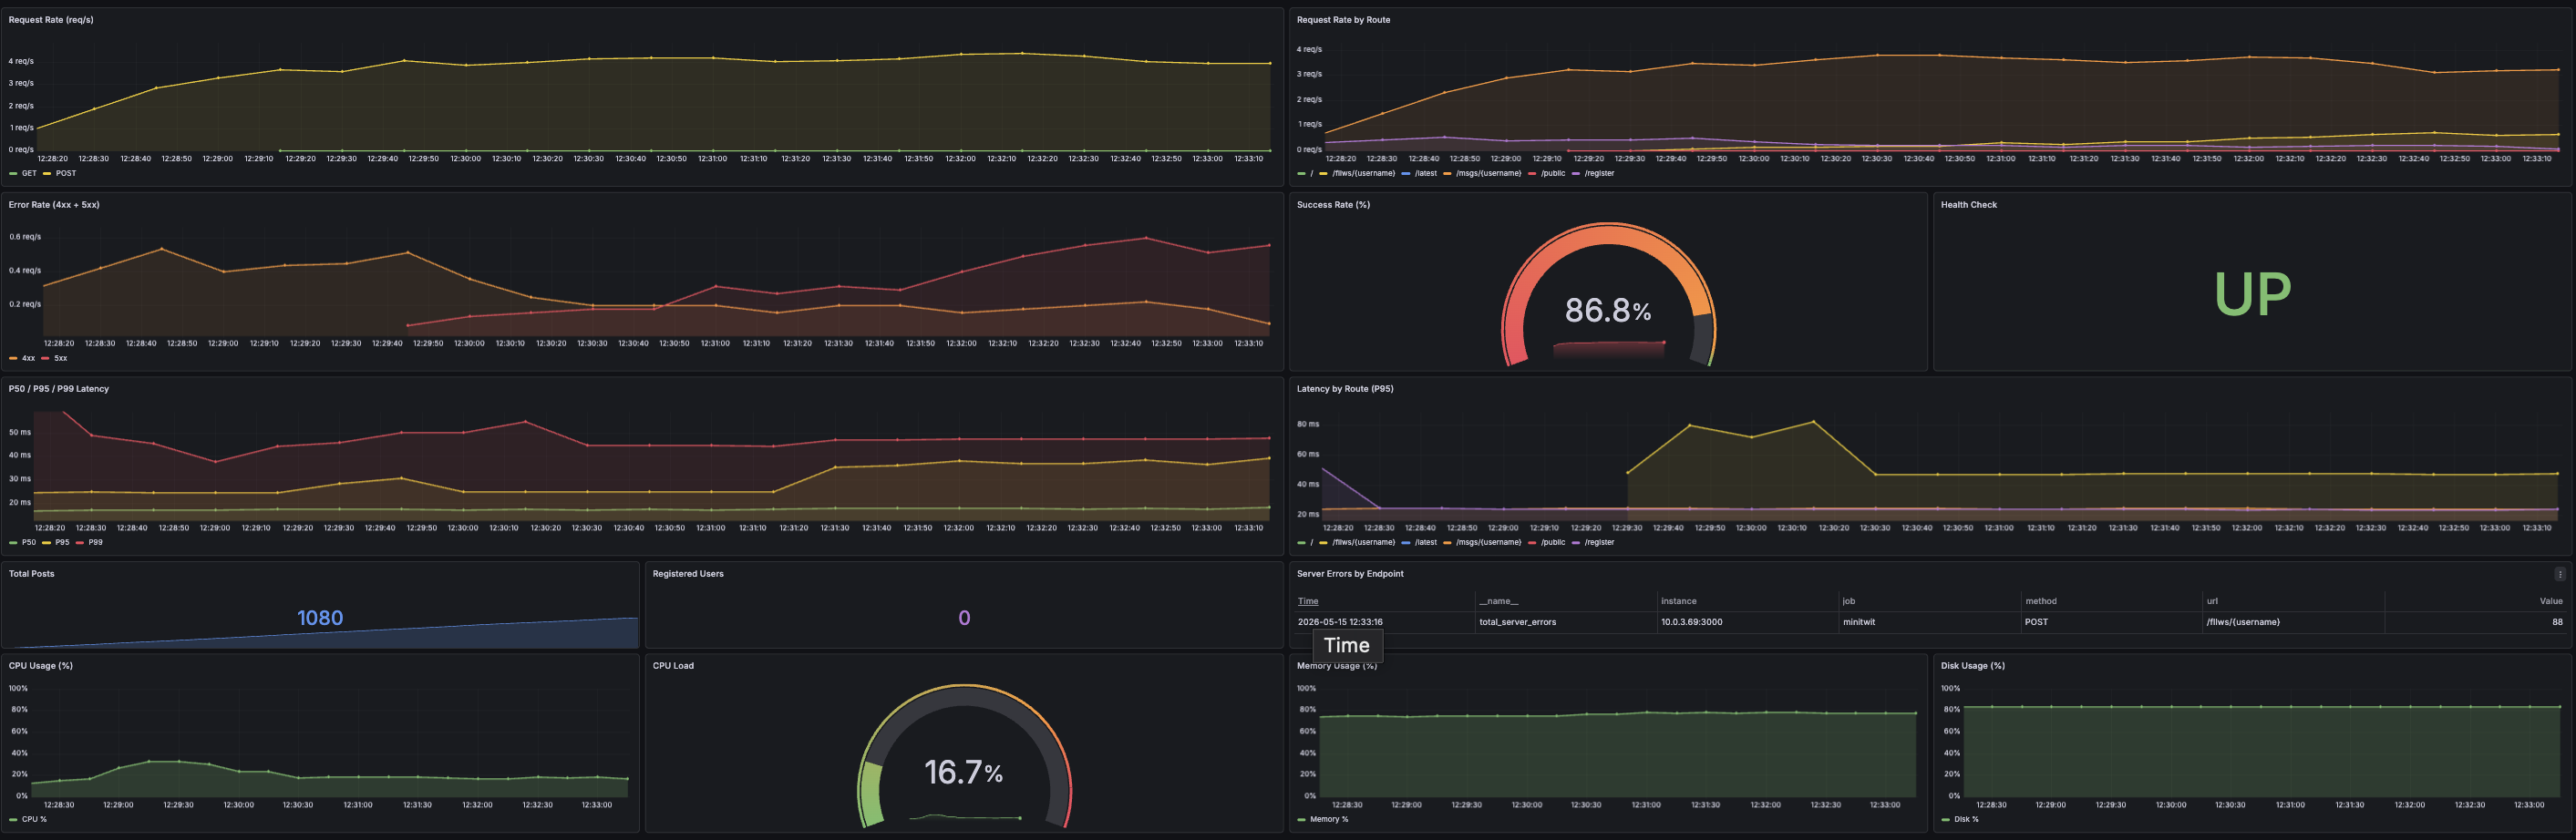
\includegraphics[width=1\textwidth]{./report/images/grafana_screen.png}
    \caption{Grafana dashboard overview}
\end{figure}

\subsection{Reflections}

The monitoring setup needs to take the deployment strategy into consideration. When switching from \texttt{docker compose} to \texttt{Docker Swarm} with multiple replicas, our scraping silently broke. Each scrape hit a different replica through Swarm's load-balancing virtual IP, so counters appeared to reset between scrapes. The solution was to use Prometheus DNS service discovery to scrape each replica separately and then sum the results in Grafana.

\section{Logging}

\subsection{Design and architecture}

Our logging pipeline uses an EFK stack (Elasticsearch, Filebeat, Kibana), as presented in the exercises. The Go web service writes structured JSON logs through \texttt{slog} to stdout. Docker captures container stdout into \texttt{/var/lib/docker/containers/} via its default JSON-file driver. Filebeat runs one instance per node in Swarm, tails those log files, decodes the Docker JSON, and ships entries directly to Elasticsearch, which stores and indexes them. Kibana sits in front for search and visualization.

The whole stack runs on its own ELK overlay network, with Caddy exposing \texttt{kibana.kulturbase.dk} over HTTPS.

\subsection{What we log}

The Go application produces structured JSON logs at multiple levels through \texttt{slog}. The HTTP middleware automatically logs every request with method, route, status, duration, and client IP. Handler-level \texttt{Logger.Error} calls add explicit context when something fails (database query, template render, JSON decode).

Container stdout from supporting services (Postgres, Caddy, Prometheus) is also captured automatically. In Kibana, we built a dashboard with four saved searches: a live error stream, a failed-request stream (\texttt{status >= 400}), a user-activity stream (registrations, logins, posts), and overall log volume by service.

\begin{figure}[h]
    \centering
    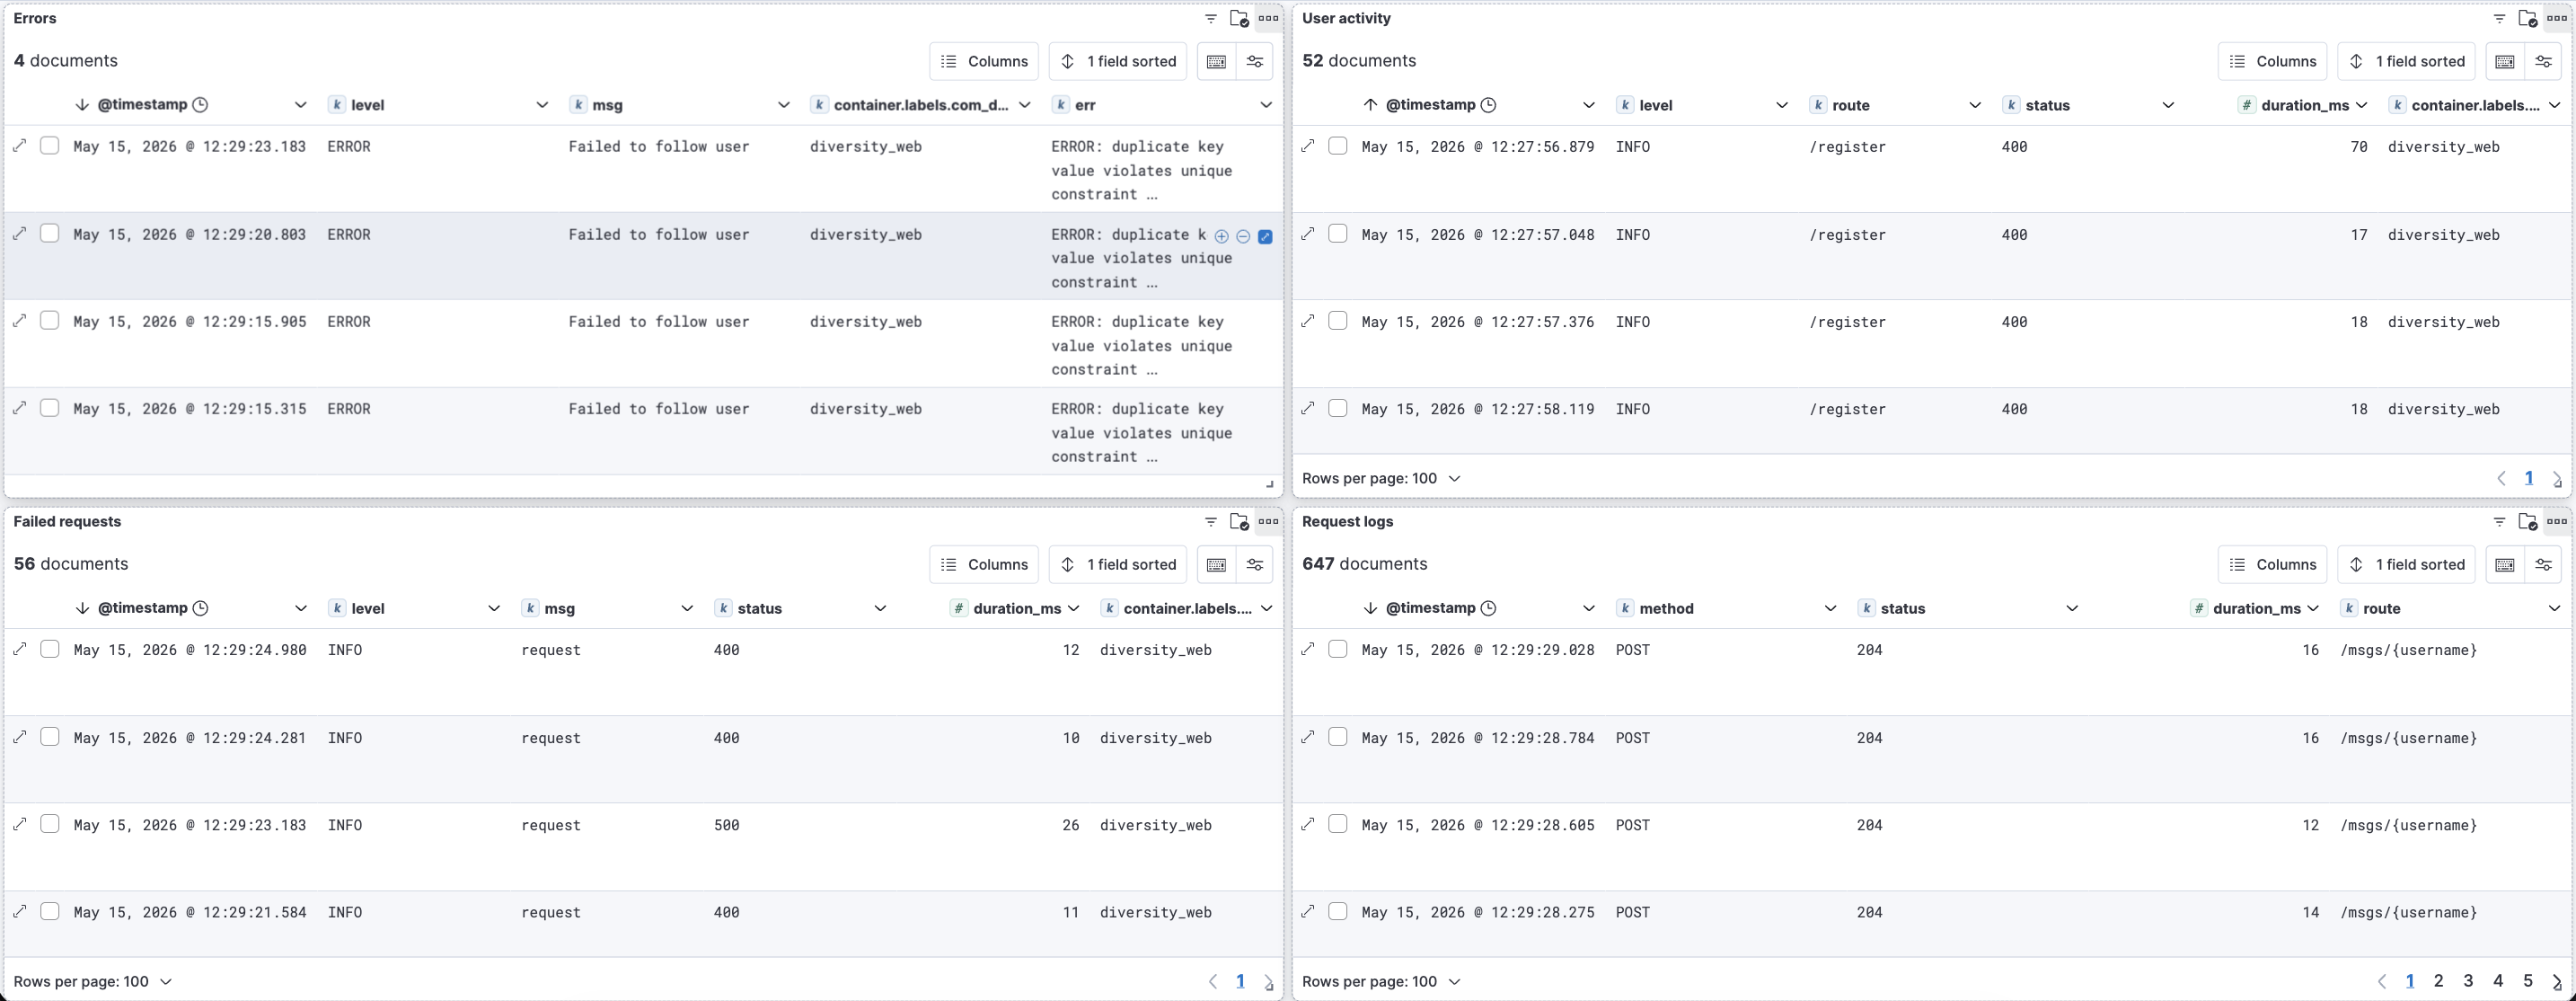
\includegraphics[width=1\textwidth]{./report/images/kibana_screen.png}
    \caption{Kibana dashboard overview}
\end{figure}

\subsection{Reflections}

Choosing the EFK stack over Grafana + Loki was, in our opinion, the wrong call for a project this small. Elasticsearch alone consumes a large amount of memory, and the stack was tricky to set up. For example, Filebeat refused to start until its configuration file was owned by root with the correct permissions, which broke our deployments until we fixed the file ownership manually on the server.

Loki would have allowed us to keep everything under one Grafana frontend, removing Kibana as a separate system to configure and manage access to. Even though it introduced unnecessary complexity, the decision was still worth it as a learning experience, since we got to try the industry-standard logging stack and encounter the kinds of real-world problems that come with it.

For a project of this size, it was overkill, but as a one-time exercise to engage with heavier tooling, it was a good choice. It also nicely separated the two concerns: Grafana tells us whether something is wrong, while Kibana explains what happened.